\sectionwithlogo{Аффинные преобразования}
	{\includeMPgraphics{figure-cat-transformed}}

%%%%%%%%%%

\begin{frame}{Определение аффинных преобразований плоскости}
\emph{Аффинные преобразования} плоскости задаются шестёркой чисел $\alert<2>{T_{xx}}$,
$\alert<2>{T_{xy}}$, $\alert<2>{T_x}$, $\alert<2>{T_{yx}}$,
$\alert<2>{T_{yy}}$, $\alert<2>{T_y}$ по формулам:
{\LARGE
	\[
	\begin{aligned}
	&\alert<3>{x'}=\alert<2>{T_{xx}}\,\alert<4>{x}+\alert<2>{T_{xy}}\,\alert<4>{y}+\alert<2>{T_x}\\
	&\alert<3>{y'}=\alert<2>{T_{yx}}\,\alert<4>{x}+\alert<2>{T_{yy}}\,\alert<4>{y}+\alert<2>{T_y}
	\end{aligned}
	\]}

\uncover<3->{\alert<3>{Новые} координаты точки выражаются через
\alert<4>{старые} линейным образом.}
\transdissolve<2->
\end{frame}

%%%%%%%%%%

\begin{frame}{Свойства аффинных преобразований}
\begin{itemize}
\item
последовательное выполнение двух аффинных преобразований равносильно некоторому
аффинному преобразованию~— их \emph{композиции}
\item
в~общем случае не \emph{коммутируют} (то есть результат композиции
преобразований зависит от порядка выполнения)
\end{itemize}
\end{frame}

%%%%%%%%%%

\begin{frame}{Невырожденность аффинных преобразований}
\emph{Невырожденным} называется аффинное преобразование, если
{\LARGE
	\[
	T_{xx}T_{yy}-T_{xy}T_{yx}\ne0.
	\]}
\end{frame}

%%%%%%%%%%

\begin{frame}{Свойства невырожденных аффинных преобразований}
\begin{itemize}
\item
прямые преобразуются в~прямые
\item
параллельные прямые преобразуются в~параллельные
\item
вполне определяется тремя точками~— вершинами треугольника, и~тремя их образами
\item
имеется \emph{обратное} преобразование, композиция с~которым оставляет все
точки плоскости на месте
\item
композиция невырожденных преобразований~— снова невырожденое
\end{itemize}
\end{frame}

%%%%%%%%%%

\begin{frame}{Кошки Арнольда}
Академик В.~И.~Арнольд очень любил кошек.

Он придумал иллюстрировать преобразования плоскости при помощи кошачьих морд.
\bigskip
\begin{center}
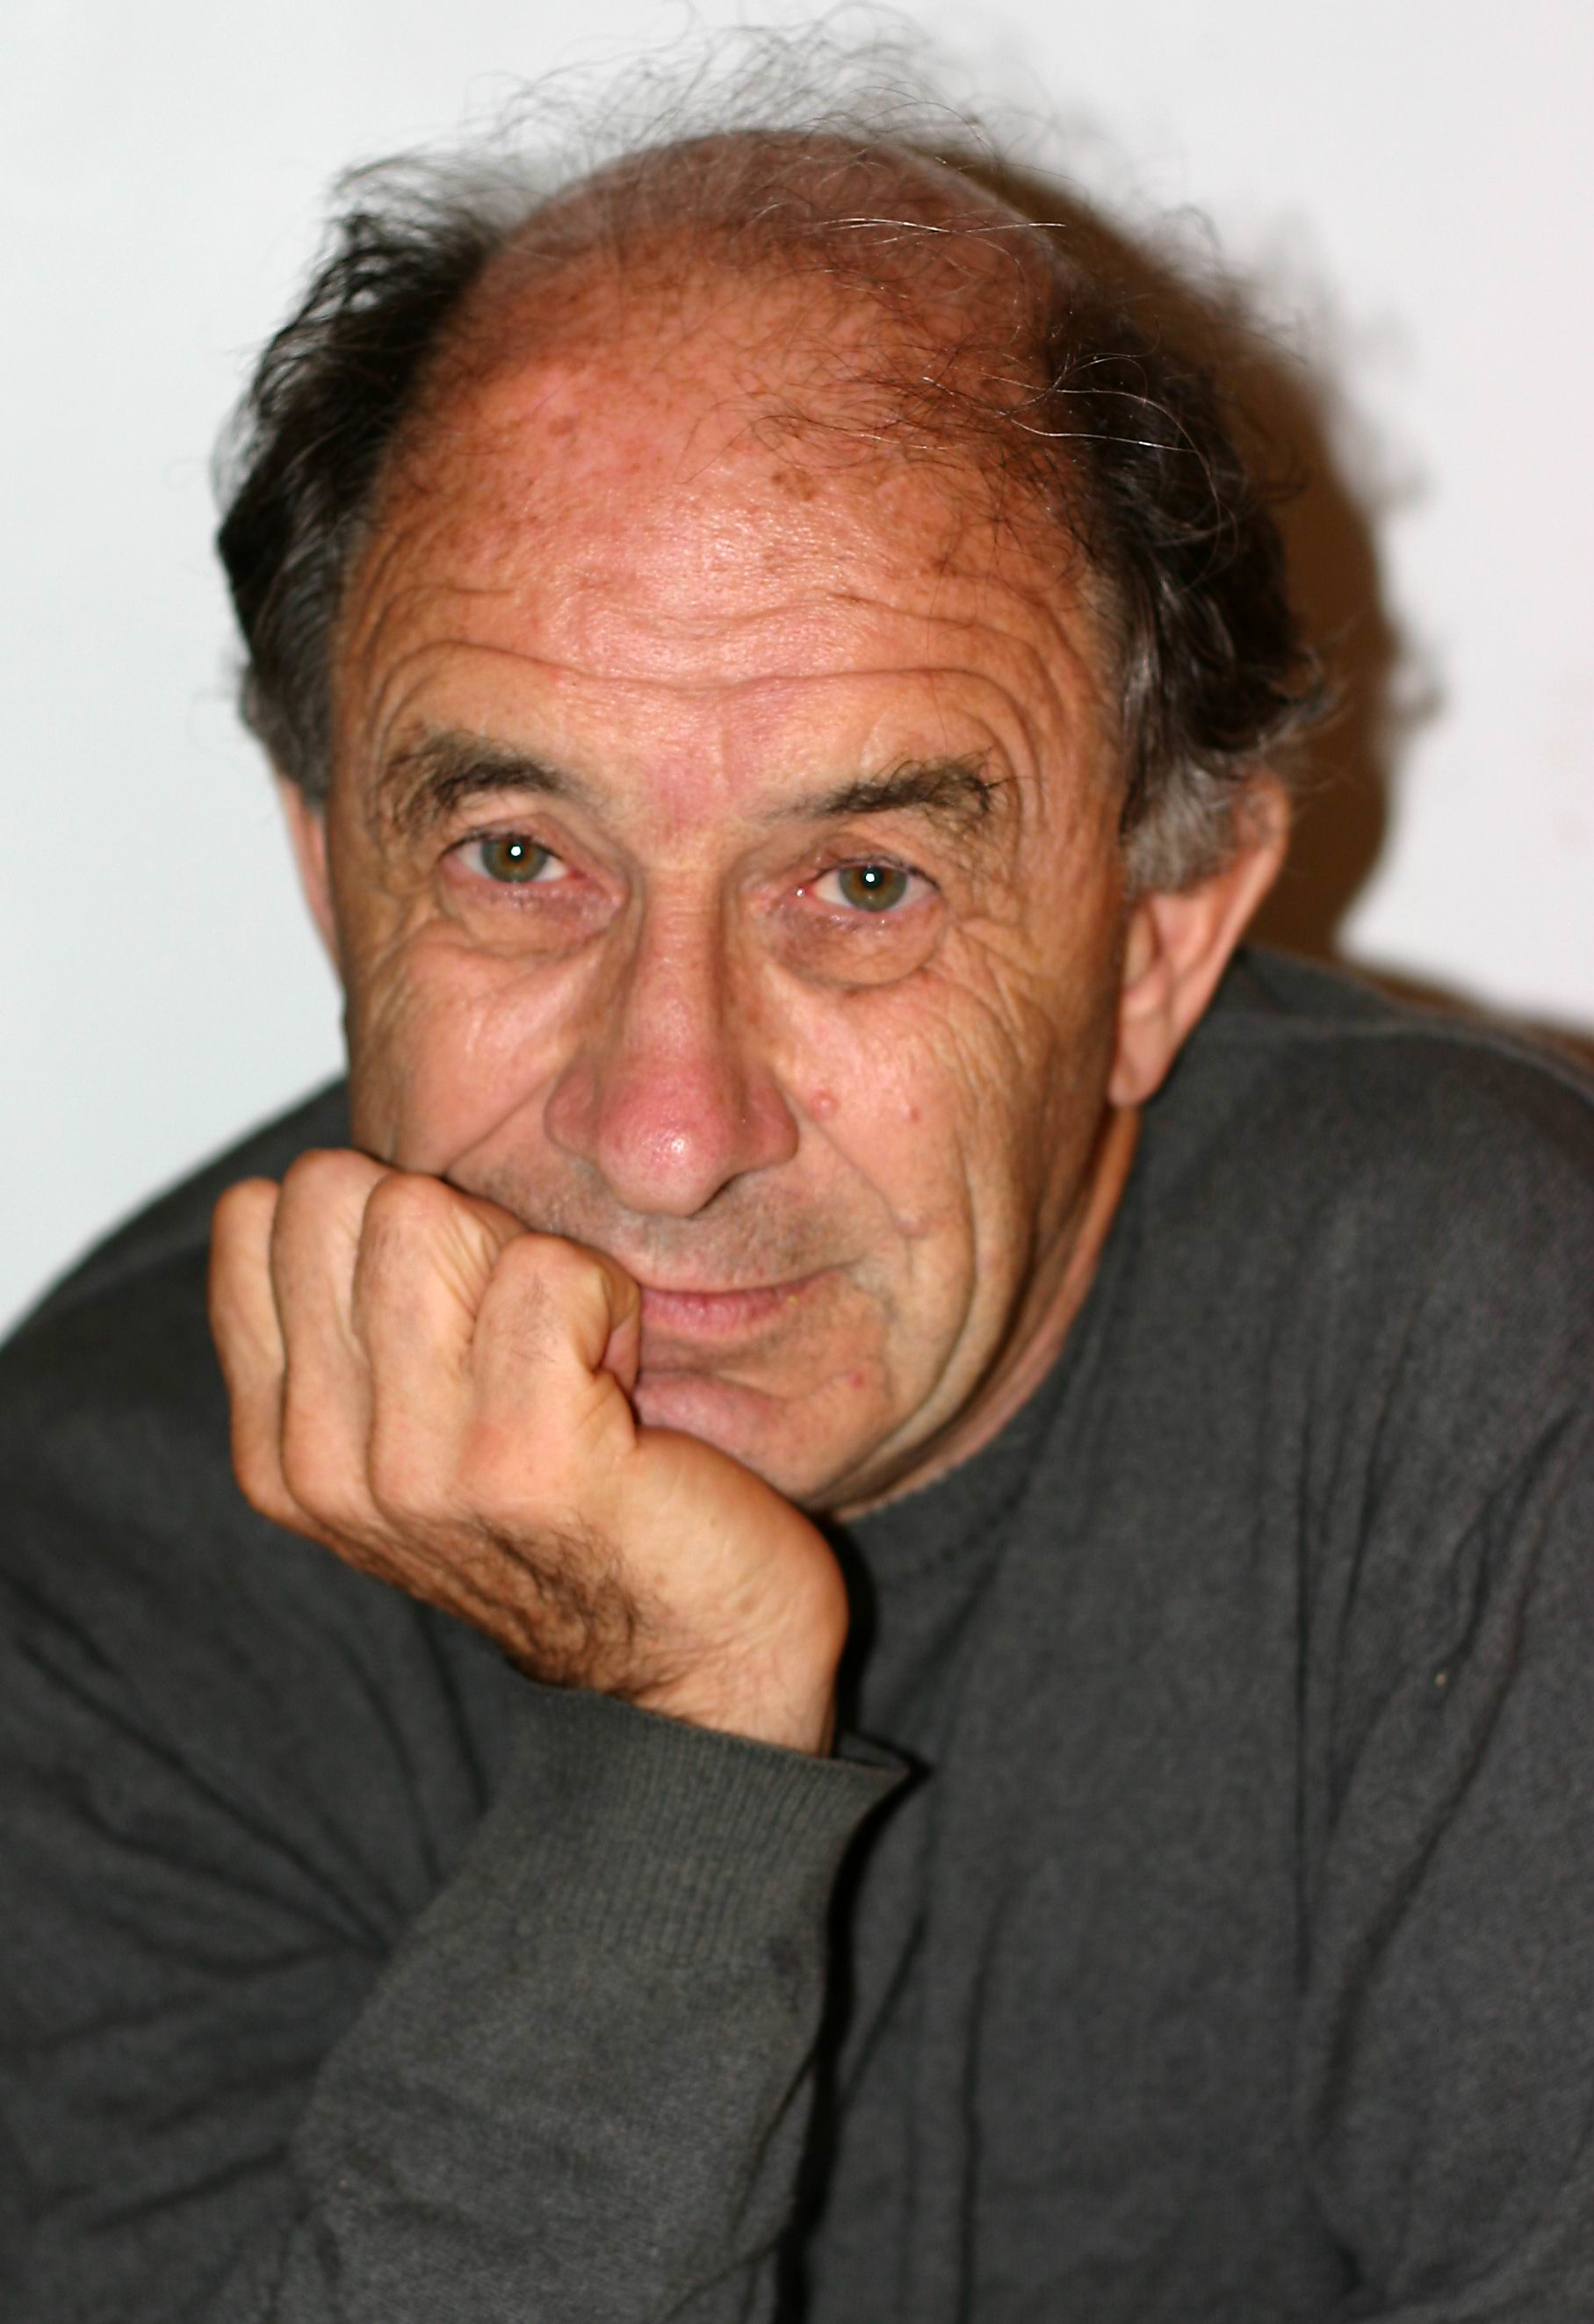
\includegraphics[height=124.874434pt]{figure-arnold}
\only<2>{\quad\includeMPgraphics{figure-cat}}
\end{center}
\end{frame}

%%%%%%%%%%

\begin{frame}{Тождественное преобразование}
\centering
\LARGE
\includeMPgraphics{figure-cat-identity}\\[4ex]
\literal{identity}
\end{frame}

%%%%%%%%%%

\begin{frame}{Сдвиг (параллельный перенос)}
\centering
\LARGE
\only<1>{\includeMPgraphics{figure-cat-shifted}\\[4ex]
\literal{identity shifted (.75, .5)}}%
\only<2>{%
$(x,y)$ \literal{shifted} $(a,b)$\\
↓\\
$(x+a,y+b)$}
\end{frame}

%%%%%%%%%%

\begin{frame}{Поворот}
\centering
\LARGE
\only<1>{\includeMPgraphics{figure-cat-rotated}\\[4ex]
\literal{identity rotated 60}}%
\only<2>{%
$(x,y)$ \literal{rotated} $\theta$\\
↓\\
$(x\cos\theta-y\sin\theta,x\sin\theta+y\cos\theta)$}
\end{frame}

%%%%%%%%%%

\begin{frame}{Растяжение}
\centering
\LARGE
\only<1>{\includeMPgraphics{figure-cat-scaled-1}}%
\only<2>{\includeMPgraphics{figure-cat-scaled-2}}%
\only<1,2>{\\[4ex]
\literal{identity scaled \only<1>{1.5}\only<2>{-.5}}}%
\only<3>{%
$(x,y)$ \literal{scaled} $k$\\
↓\\
$(kx,ky)$}
\end{frame}

%%%%%%%%%%

\begin{frame}{Дилатация~— растяжение по~\only<1,2>{горизонтали}\only<3,4>{вертикали}}
\centering
\LARGE
\only<1>{\includeMPgraphics{figure-cat-xscaled}}%
\only<3>{\includeMPgraphics{figure-cat-yscaled}}%
\only<1,3>{\\[4ex]
\literal{identity \only<1>{\alert{x}scaled 2.5}\only<3>{\alert{y}scaled .25}}}%
\only<2,4>{%
$(x,y)$ \literal{\only<2>{x}\only<4>{y}scaled} $k$\\
↓\\
$(\only<2>{k}x,\only<4>{k}y)$}
\end{frame}

%%%%%%%%%%

\begin{frame}{Растяжение с~поворотом}
\centering
\LARGE
\only<1>{\includeMPgraphics{figure-cat-zscaled}}%
\only<1>{\\[4ex]
\literal{identity \alert{z}scaled (1.2, .5)}}%
\only<2,3>{%
$(x,y)$ \literal{zscaled} $(u,v)$\\
↓\\
\only<2>{$(xu-yv,xv+yu)$}%
\only<3>{$(x,y)$ \literal{scaled abs} $(u,v)$ \literal{rotated angle} $(u,v)$}}
\transdissolve<3->
\end{frame}

%%%%%%%%%%

\begin{frame}{Растяжение с~поворотом}
Кстати, поворот на $90^\circ$ (по или против часовой стрелки) проще
и~эффективнее задать как \literal{zscaled up} или \literal{zscaled down} вместо
\literal{rotated 90} или \literal{rotated -90} соответственно~— тогда не будут
вычисляться тригонометрические функции.

Поворот на $180^\circ$ лучше задать как \literal{zscaled left}.
\end{frame}

%%%%%%%%%%

\begin{frame}{Наклон}
\centering
\LARGE
\only<1>{\includeMPgraphics{figure-cat-slanted}\\[4ex]
\literal{identity slanted 2}}%
\only<2>{%
$(x,y)$ \literal{slanted} $k$\\
↓\\
$(x+ky,y)$}
\end{frame}

%%%%%%%%%%

\begin{frame}{Поворот вокруг заданной точки}
\centering
\LARGE
\only<1>{\includeMPgraphics{figure-cat-rotatedabout}%
\\[4ex]
\literal{identity}\par
\literal{rotatedabout((1, 1), 90)}}%
\only<2>{%
$p$ \literal{rotatedabout(}$z$\literal{, }$\theta$\literal{)}\\
↓\\
$p$ \literal{shifted} $-z$ \literal{rotated} $\theta$ \literal{shifted} $z$}
\end{frame}

%%%%%%%%%%

\begin{frame}{Осевая симметрия (зеркальное отражение)}
\centering
\includeMPgraphics{figure-cat-reflectedabout}\\[4ex]
\LARGE
\literal{identity}\par
\literal{reflectedabout((0, .5), (1, 1))}
\end{frame}

%%%%%%%%%%

\begin{frame}{Композиция аффинных преобразований}
\centering
\includeMPgraphics{figure-cat-transformed}\\[4ex]
\LARGE
\literal{identity scaled .8 rotated -30}\par
\literal{slanted .5 shifted (.5, .25)}
\end{frame}

%%%%%%%%%%

\begin{frame}{Преобразование, заданное своими коэффициентами}
\centering
\LARGE
$(x,y)$ \literal{transformed} $(T_x,T_y,T_{xx},T_{xy},T_{yx},T_{yy})$\\
↓\\
$(T_x+T_{xx}\,x+T_{xy}\,y,T_y+T_{yx}\,x+T_{yy}\,y)$
\end{frame}

%%%%%%%%%%

\begin{frame}{Декомпозиция аффинных преобразований}
Отдельные компоненты аффинного преобразования
$T=(T_x,T_y,T_{xx},T_{xy},T_{yx},T_{yy})$ можно получить при помощи операторов
\literal{xpart}, \literal{ypart}, \literal{xxpart}, \literal{xypart},
\literal{yxpart}, \literal{yypart}:

\begin{center}
\begin{tabular}{r@{\enspace→\enspace}l}
\literal{xpart} $T$&$T_x$\\
\literal{ypart} $T$&$T_y$\\
\literal{xxpart} $T$&$T_{xx}$\\
\literal{xypart} $T$&$T_{xy}$\\
\literal{yxpart} $T$&$T_{yx}$\\
\literal{yypart} $T$&$T_{yy}$
\end{tabular}
\end{center}
\end{frame}

%%%%%%%%%%

\begin{frame}{Обратное преобразование}
Преобразование~$T'$, обратное к~$T$, вычисляет оператор \literal{inverse}:

\begin{center}
\begin{tabular}{r@{\enspace→\enspace}l}
\literal{inverse} $T$&$T'$\\
\end{tabular}
\end{center}
\end{frame}
